\subsection{Step 5: test leading and next powers from CFT}
\label{sec:complement-theory}
The analytical source is \texttt{manuscript\_theory/main3.tex}
\cite{theoryLarge}. Its compiled \texttt{main.pdf} is an older version
without the worked examples used here. In the mixing operator product
expansion, let $\Delta$ be the lowest exchanged scaling dimension and
$c_{ab}$ its normalized coefficient. At $p=1/2$ the leading deficit is
\begin{equation}
 \delta_{a\mid b}(y)=B_{ab}y^{\beta_{\rm CFT}}+\cdots,\qquad
 \beta_{\rm CFT}=2\Delta,\qquad
 B_{ab}=\pi^{2\Delta}|c_{ab}|^2
 \frac{\sqrt\pi\,\Gamma(1+\Delta)}{4\Gamma(3/2+\Delta)}.
 \label{eq:complement-leading}
\end{equation}
$\Gamma$ is Euler's gamma function. In particular, $B_{ab}$ includes
$\pi^{\beta_{\rm CFT}}$. Each leading coefficient is shared by the
two directions; their higher-order coefficients need not coincide.
\begin{table}[htbp]\centering\small
\begin{tabular}{llccc}\toprule
CFT & Pair (both directions) & $\beta_{\rm CFT}$ & $B_{ab}$ & Next power\\\midrule
Ising & $I,\sigma$ & $1/4$ & $\pi^{3/4}\Gamma(9/8)/[4\Gamma(13/8)]$ & $1/2$\\
Ising & $I,\eps$ & $2$ & $\pi^2/3$ & $4$\\
Ising & $\sigma,\eps$ & $1/4$ & $\pi^{3/4}\Gamma(9/8)/[16\Gamma(13/8)]$ & $1/2$\\
Boson & $00,ss$ & $1$ & $\pi^2/8$ & $2$\\
Boson & $00,3s,s$ & $5$ & $5\pi^6/64$ & $6$\\
Boson & $ss,3s,s$ & $2$ & $\pi^2/3$ & $3$ (allowed)\\\bottomrule
\end{tabular}
\caption{Leading large-interval amplitudes multiplying $y^\beta$ and
next powers used in $F_2$, at $p=1/2$ and $s=1/\sqrt2$.
The Ising spin--energy channel includes $|c_{\sigma\eps}|^2=1/4$.
For boson charge codes $(a_i,b_i)$,
$\Delta=[(a_1-a_2)^2+(b_1-b_2)^2]/4$ and $|c_{ab}|=1$.
The last next power follows from the manuscript's general three-point
sector rather than a separately evaluated example; its coefficient may
vanish. No next-order coefficient is supplied or derived here.}
\label{tab:complement-theory}
\end{table}

The manuscript's Ising examples explicitly identify four-spin terms
of order $y^{1/2}$ and later two-spin--energy terms of order $y^{5/4}$;
the first correction retained in $F_2$ is $y^{1/2}$. The identity--energy
example specifies a remainder of order $y^4$. The boson vacuum examples
specify orders $y^2$ and $y^6$. For the remaining boson pair, the general
subsection ``Three point function'' contains powers
$2\Delta_{L'}+\Delta_L$: the exchanged vertex has $\Delta_{L'}=1$
and a current has $\Delta_L=1$, giving the candidate power three.
This identifies an allowed sector, not a proved nonzero total
coefficient after replica continuation. We consequently interpret
that pair's $F_2$ as a test of the next allowed power. This qualification
also prevents an $O(y^r)$ remainder from being mistaken for a known
coefficient. No universal increment of two is imposed for large intervals.

\begin{equation}
 F_{\rm free}(y)=Cy^{\widehat\beta},\qquad
 F_1(y)=c_0y^{\beta_{\rm CFT}},\qquad
 F_2(y)=c_0y^{\beta_{\rm CFT}}+c_1y^{\beta_1}.
 \label{eq:complement-fit}
\end{equation}
Here $\beta_1$ is the next power in Table~\ref{tab:complement-theory}.
Only the exponents of $F_1,F_2$ are imposed; all their coefficients
are fitted separately in each direction. ``CFT leading'' always means
$B_{ab}y^{\beta_{\rm CFT}}$, with neither parameter fitted.
For completeness, the one-term solution is
\begin{equation}
 c_0=\frac{\sum_i y_i^{\beta_{\rm CFT}}\delta_i}
                 {\sum_i y_i^{2\beta_{\rm CFT}}}.
 \label{eq:complement-fixed-fit}
\end{equation}
The fits use the CFT-wide windows in Eq.~\eqref{eq:common-fit-windows}:
$y\leq0.002$ for Ising and $y\leq0.005$ for the boson. Every
direction uses the same window as its reverse. Figures show data
through $y\leq0.20$, with fitting-window zooms in the per-pair views.
The objective, coefficient convention, residuals and size cross-validation
are exactly Eqs.~\eqref{eq:objective}, \eqref{eq:metrics} and \eqref{eq:cv}.
\begin{equation}
 R_i=100[\delta_i-M(y_i)]/\delta_i,\qquad
 \eta_\beta=100(\widehat\beta/\beta_{\rm CFT}-1).
 \label{eq:complement-fit-metrics}
\end{equation}
\begin{equation}
 \mathrm{CVRMSE}=\sqrt{m^{-1}\sum_i[\delta_i-M^{(-N_i)}(y_i)]^2}.
 \label{eq:complement-cv}
\end{equation}
The residual sign in the entropy $D^B=\log2-\delta$ is opposite to
the deficit residual. Tables in Appendix~\ref{sec:complement-checks}
separate Free, $F_1$, $F_2$ and CFT rows for all twelve directions.
\subsection{Results}
\label{sec:complement-results}
Ising full-window free-exponent deviations range from $-0.074\%$ to $+5.861\%$. $F_2$ improves size-holdout RMSE over $F_1$ in 6 of six directions. These statements use the prescribed fitting window and the sample-count requirements in Appendix~\ref{sec:window-comparison}.\par
Compact-boson full-window free-exponent deviations range from $-0.438\%$ to $-0.074\%$. $F_2$ improves size-holdout RMSE over $F_1$ in 2 of six directions. These statements use the prescribed fitting window and the sample-count requirements in Appendix~\ref{sec:window-comparison}.\par

\begin{figure}[p]\centering
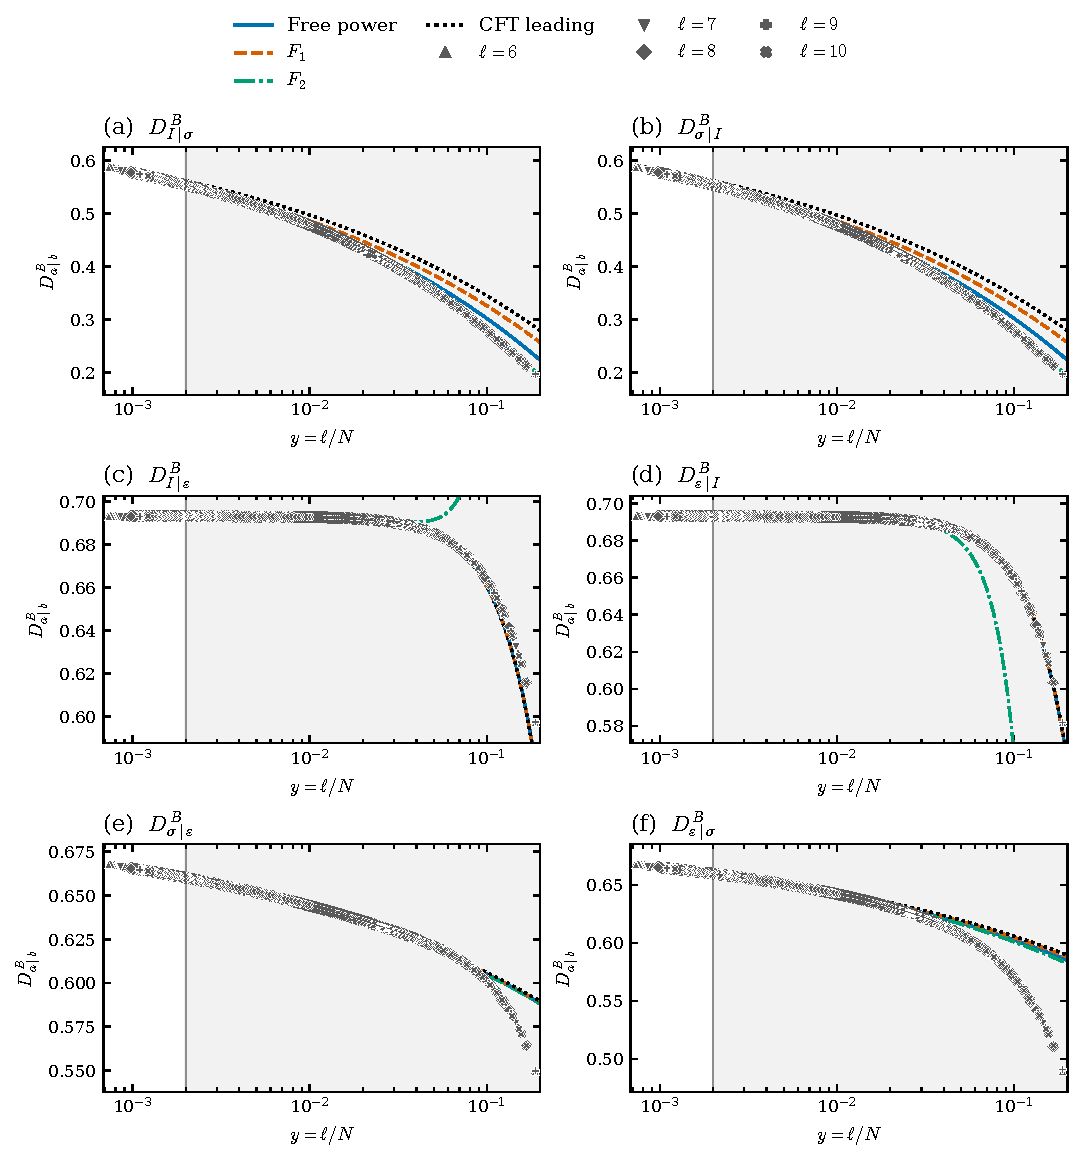
\includegraphics[width=.88\linewidth]{../figs/ising_large_entropy.pdf}
\caption{The ordinate is $D^B=\log2-\delta$, on a linear scale; tick labels give its value directly, without an additive offset. The fraction axis is logarithmic. Ising mixtures at $p=1/2$, $\ell=6,7,8,9,10$, and the chain-size set in Eq.~\eqref{eq:extended-grid}, with $32\leq N\leq8192$. There are 1645 displayed geometries per direction at $y\leq0.2$, of which 260 satisfy $y\leq0.002$ and enter every fit. Marker shape identifies $\ell$; the vertical boundary and gray shading mark the fitting cutoff and excluded data. The periodic Ising Hamiltonian is $H=-\sum_jX_jX_{j+1}-\sum_jZ_j$; primaries use exact fermionic covariances, including the odd Ramond ground state for $\sigma$. Natural logarithms apply. Added sizes use the direct entropy remainder in Sec.~\ref{sec:stable-entropy}, with support cutoff $10^{-15}$. Blue solid is the free-power fit (two fitted parameters), orange dashed is $F_1$ (one), green dash--dot is $F_2$ (two), and black dotted is the analytical CFT leading term (zero). Powers and amplitudes use Eqs.~\eqref{eq:fit} and \eqref{eq:complement-fit}; all coefficients include powers of $\pi$. Fits minimize unweighted squared residuals in $\delta$. These curves use \texttt{scaling\_fit\_summary.csv}. The identical fits in Tables~\ref{tab:ising-large-parameters} and \ref{tab:ising-large-metrics} also have per-pair full-range and fitting-window views in Sec.~\ref{sec:pair-large_ising}.}
\label{fig:ising-complement-entropy}
\end{figure}

\begin{figure}[p]\centering
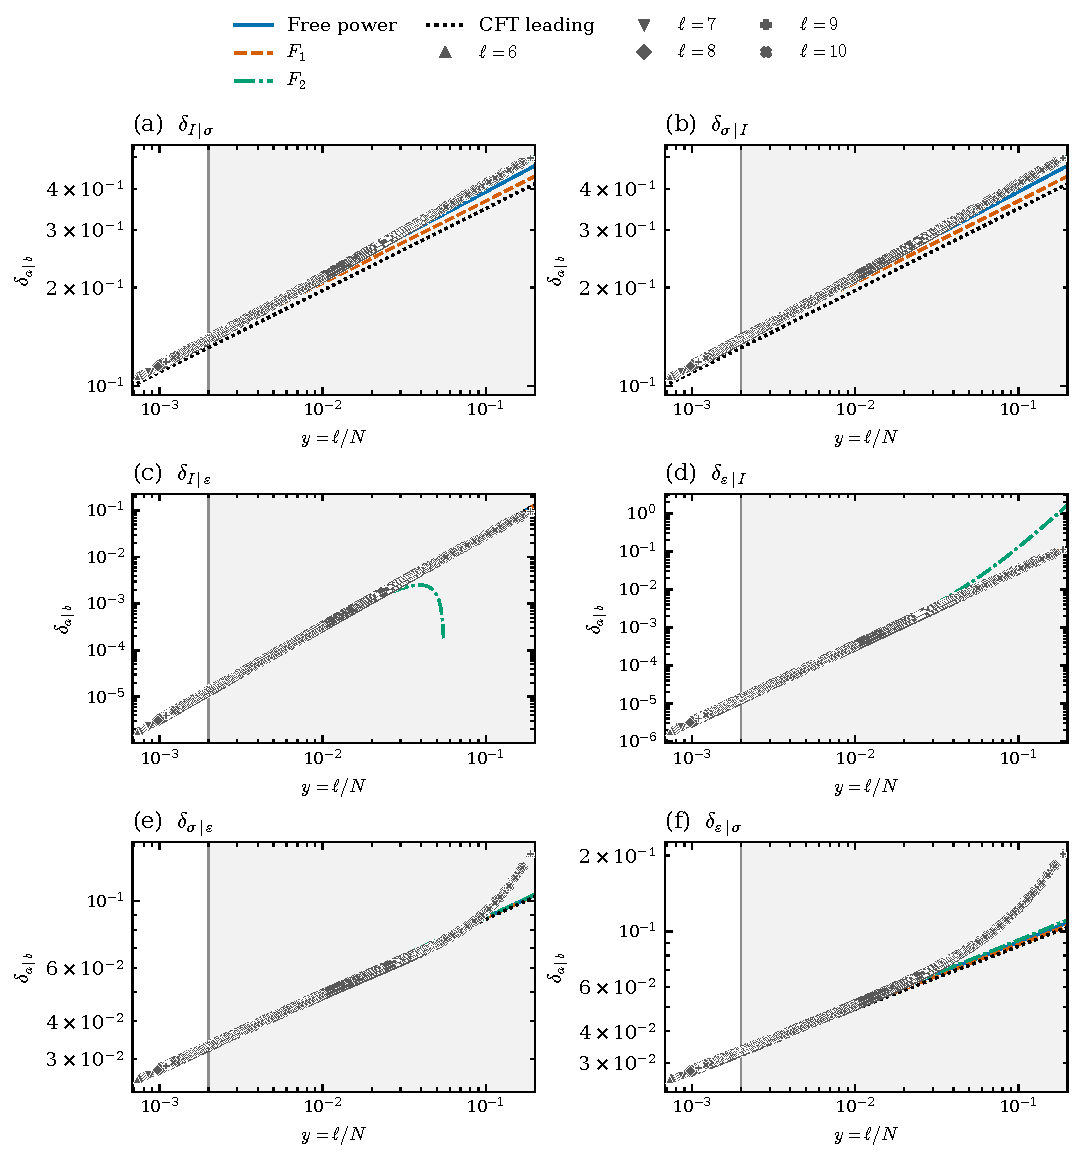
\includegraphics[width=.88\linewidth]{../figs/ising_large_value.pdf}
\caption{Both axes are logarithmic. Nonpositive values of an extrapolated truncated curve are omitted only from this logarithmic panel, while residual panels retain their predictions. Ising mixtures at $p=1/2$, $\ell=6,7,8,9,10$, and the chain-size set in Eq.~\eqref{eq:extended-grid}, with $32\leq N\leq8192$. There are 1645 displayed geometries per direction at $y\leq0.2$, of which 260 satisfy $y\leq0.002$ and enter every fit. Marker shape identifies $\ell$; the vertical boundary and gray shading mark the fitting cutoff and excluded data. The periodic Ising Hamiltonian is $H=-\sum_jX_jX_{j+1}-\sum_jZ_j$; primaries use exact fermionic covariances, including the odd Ramond ground state for $\sigma$. Natural logarithms apply. Added sizes use the direct entropy remainder in Sec.~\ref{sec:stable-entropy}, with support cutoff $10^{-15}$. Blue solid is the free-power fit (two fitted parameters), orange dashed is $F_1$ (one), green dash--dot is $F_2$ (two), and black dotted is the analytical CFT leading term (zero). Powers and amplitudes use Eqs.~\eqref{eq:fit} and \eqref{eq:complement-fit}; all coefficients include powers of $\pi$. Fits minimize unweighted squared residuals in $\delta$. These curves use \texttt{scaling\_fit\_summary.csv}. The identical fits in Tables~\ref{tab:ising-large-parameters} and \ref{tab:ising-large-metrics} also have per-pair full-range and fitting-window views in Sec.~\ref{sec:pair-large_ising}.}
\label{fig:ising-complement-deficit}
\end{figure}

\begin{figure}[p]\centering
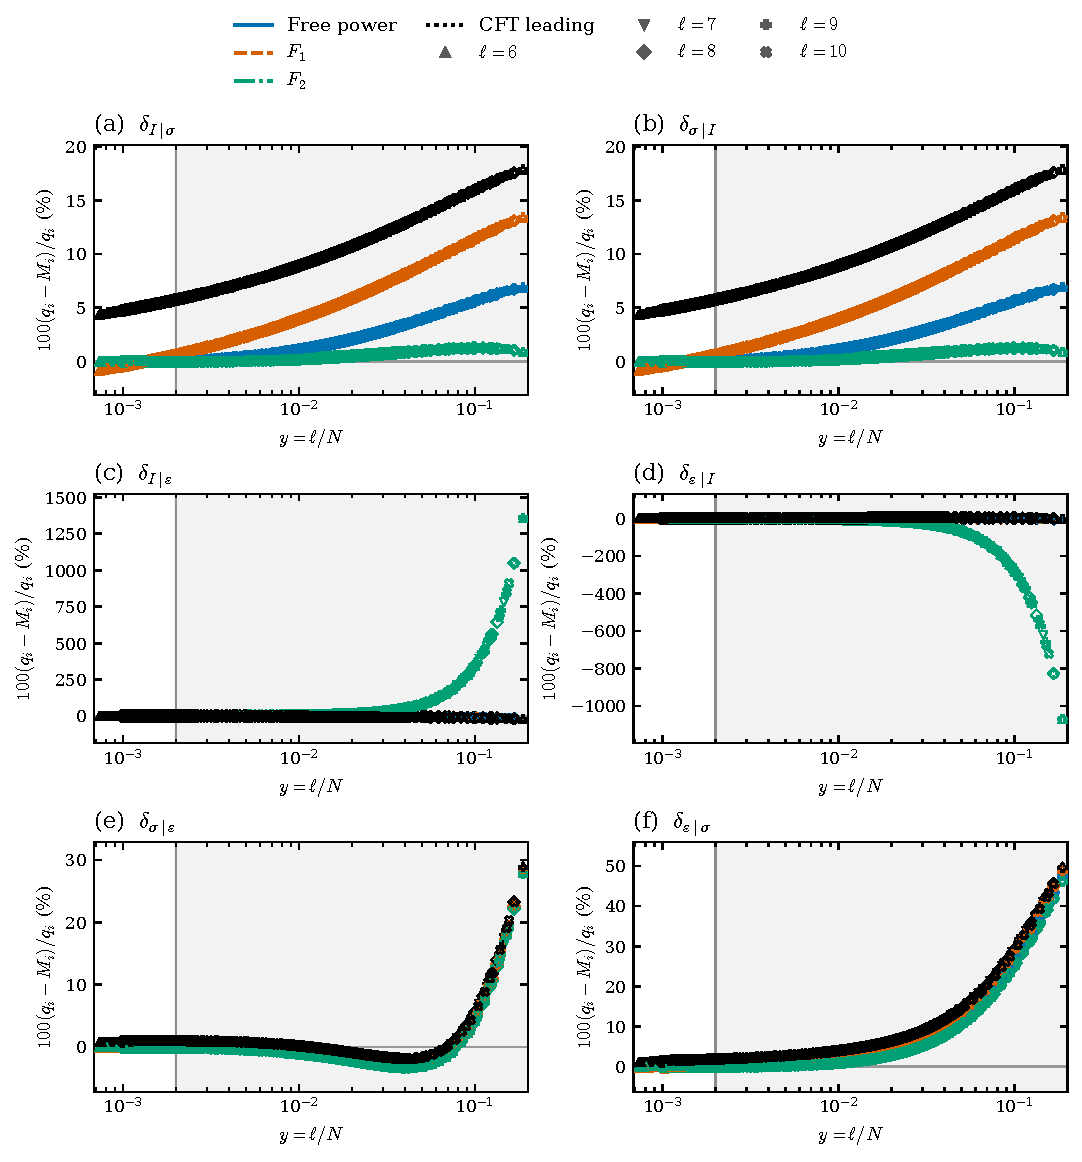
\includegraphics[width=.88\linewidth]{../figs/ising_large_residual.pdf}
\caption{The ordinate is $100(q_i-M_i)/q_i$ percent, with $q_i=D^A_i$ for a small interval and $q_i=\delta_i$ for a large interval; the horizontal zero line aids comparison. All four models have residual markers, colored as their curves. The residual ordinate is linear; the fraction axis is logarithmic. Ising mixtures at $p=1/2$, $\ell=6,7,8,9,10$, and the chain-size set in Eq.~\eqref{eq:extended-grid}, with $32\leq N\leq8192$. There are 1645 displayed geometries per direction at $y\leq0.2$, of which 260 satisfy $y\leq0.002$ and enter every fit. Marker shape identifies $\ell$; the vertical boundary and gray shading mark the fitting cutoff and excluded data. The periodic Ising Hamiltonian is $H=-\sum_jX_jX_{j+1}-\sum_jZ_j$; primaries use exact fermionic covariances, including the odd Ramond ground state for $\sigma$. Natural logarithms apply. Added sizes use the direct entropy remainder in Sec.~\ref{sec:stable-entropy}, with support cutoff $10^{-15}$. Blue solid is the free-power fit (two fitted parameters), orange dashed is $F_1$ (one), green dash--dot is $F_2$ (two), and black dotted is the analytical CFT leading term (zero). Powers and amplitudes use Eqs.~\eqref{eq:fit} and \eqref{eq:complement-fit}; all coefficients include powers of $\pi$. Fits minimize unweighted squared residuals in $\delta$. These curves use \texttt{scaling\_fit\_summary.csv}. The identical fits in Tables~\ref{tab:ising-large-parameters} and \ref{tab:ising-large-metrics} also have per-pair full-range and fitting-window views in Sec.~\ref{sec:pair-large_ising}.}
\label{fig:ising-complement-residuals}
\end{figure}

\begin{figure}[p]\centering
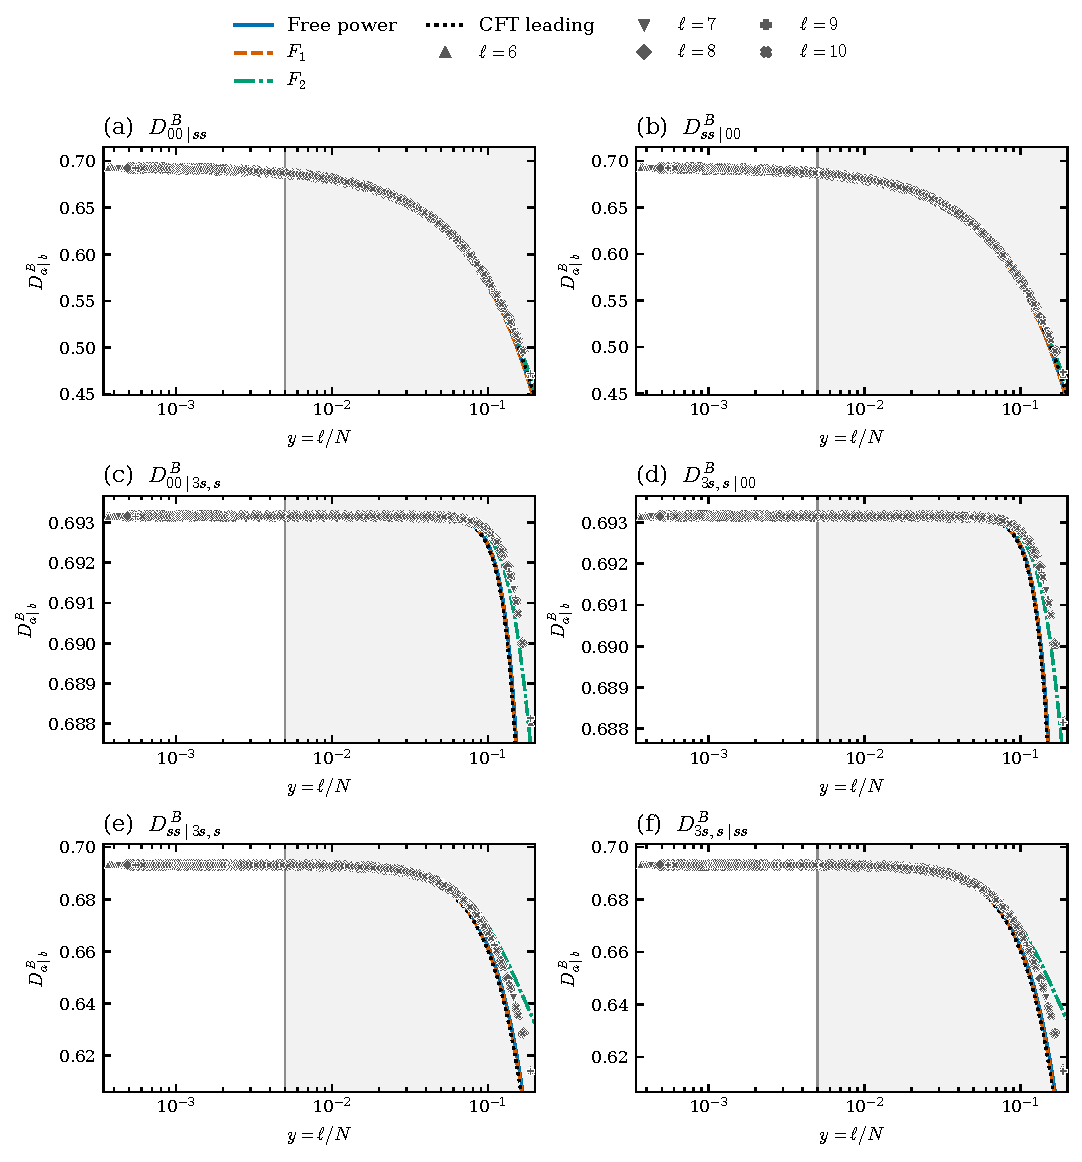
\includegraphics[width=.88\linewidth]{../figs/boson_large_entropy.pdf}
\caption{The ordinate is $D^B=\log2-\delta$, on a linear scale; tick labels give its value directly, without an additive offset. The fraction axis is logarithmic. Compact-boson mixtures at $p=1/2$, $\ell=6,7,8,9,10$, and the chain-size set in Eq.~\eqref{eq:extended-grid}, with $32\leq N\leq16384$. There are 625 displayed geometries per direction at $y\leq0.2$, of which 317 satisfy $y\leq0.005$ and enter every fit. Marker shape identifies $\ell$; the vertical boundary and gray shading mark the fitting cutoff and excluded data. The boson uses $s=1/\sqrt2$, $q=2$, charge codes $(0,0),(1,1),(3,1)$, $z_j=e^{2\pi i j/N}$, $w_1=0$, and $W=10^8$; moment algebra uses 100 digits through $N=256$ and 120 digits at the added sizes. Natural logarithms apply. Added sizes use the direct entropy remainder in Sec.~\ref{sec:stable-entropy}, with support cutoff $10^{-15}$. Blue solid is the free-power fit (two fitted parameters), orange dashed is $F_1$ (one), green dash--dot is $F_2$ (two), and black dotted is the analytical CFT leading term (zero). Powers and amplitudes use Eqs.~\eqref{eq:fit} and \eqref{eq:complement-fit}; all coefficients include powers of $\pi$. Fits minimize unweighted squared residuals in $\delta$. These curves use \texttt{scaling\_fit\_summary.csv}. The identical fits in Tables~\ref{tab:boson-large-parameters} and \ref{tab:boson-large-metrics} also have per-pair full-range and fitting-window views in Sec.~\ref{sec:pair-large_boson}.}
\label{fig:boson-complement-entropy}
\end{figure}

\begin{figure}[p]\centering
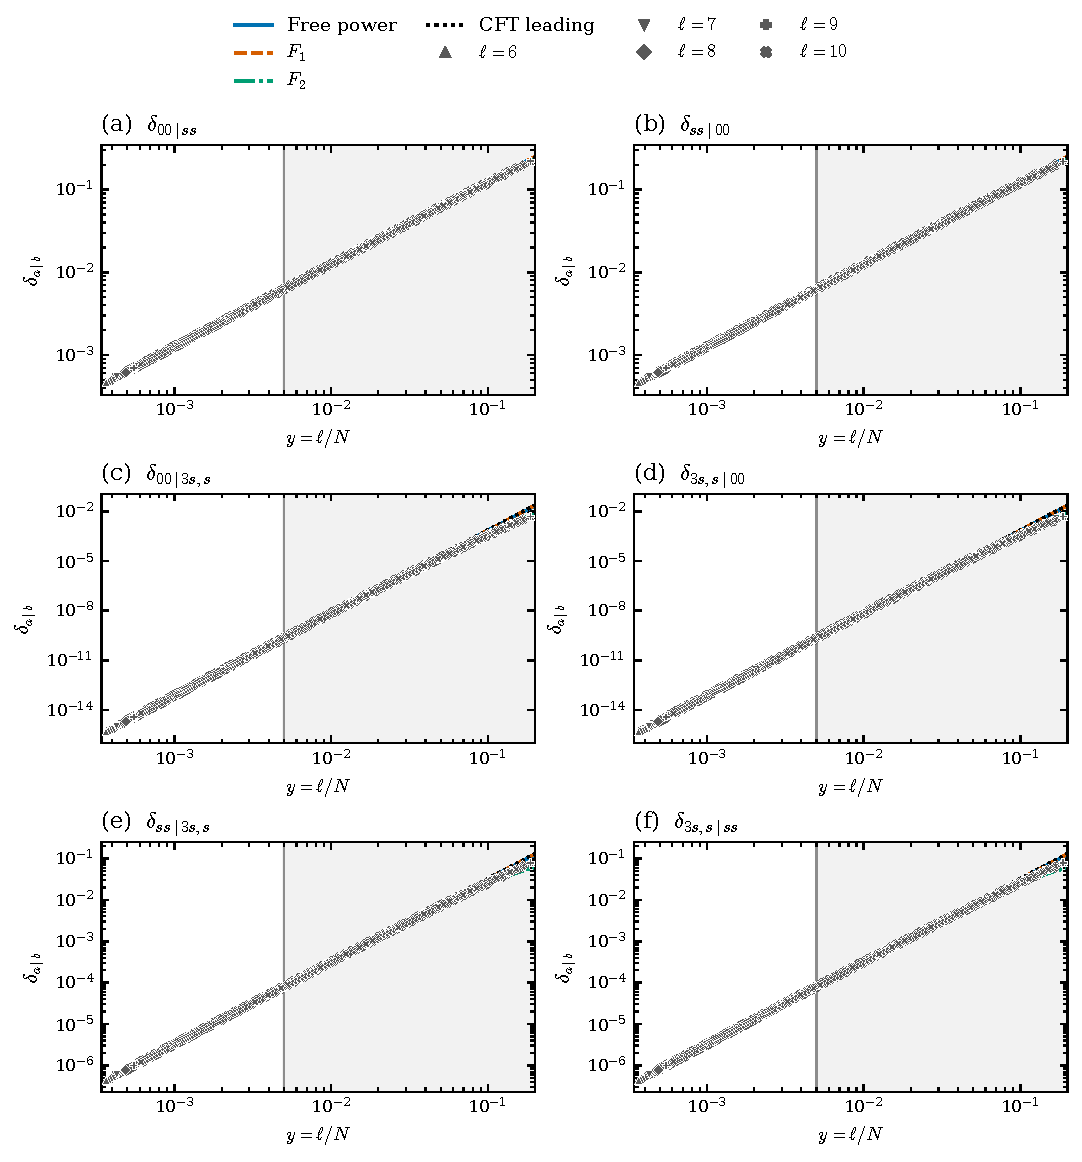
\includegraphics[width=.88\linewidth]{../figs/boson_large_value.pdf}
\caption{Both axes are logarithmic. Nonpositive values of an extrapolated truncated curve are omitted only from this logarithmic panel, while residual panels retain their predictions. Compact-boson mixtures at $p=1/2$, $\ell=6,7,8,9,10$, and the chain-size set in Eq.~\eqref{eq:extended-grid}, with $32\leq N\leq16384$. There are 625 displayed geometries per direction at $y\leq0.2$, of which 317 satisfy $y\leq0.005$ and enter every fit. Marker shape identifies $\ell$; the vertical boundary and gray shading mark the fitting cutoff and excluded data. The boson uses $s=1/\sqrt2$, $q=2$, charge codes $(0,0),(1,1),(3,1)$, $z_j=e^{2\pi i j/N}$, $w_1=0$, and $W=10^8$; moment algebra uses 100 digits through $N=256$ and 120 digits at the added sizes. Natural logarithms apply. Added sizes use the direct entropy remainder in Sec.~\ref{sec:stable-entropy}, with support cutoff $10^{-15}$. Blue solid is the free-power fit (two fitted parameters), orange dashed is $F_1$ (one), green dash--dot is $F_2$ (two), and black dotted is the analytical CFT leading term (zero). Powers and amplitudes use Eqs.~\eqref{eq:fit} and \eqref{eq:complement-fit}; all coefficients include powers of $\pi$. Fits minimize unweighted squared residuals in $\delta$. These curves use \texttt{scaling\_fit\_summary.csv}. The identical fits in Tables~\ref{tab:boson-large-parameters} and \ref{tab:boson-large-metrics} also have per-pair full-range and fitting-window views in Sec.~\ref{sec:pair-large_boson}.}
\label{fig:boson-complement-deficit}
\end{figure}

\begin{figure}[p]\centering
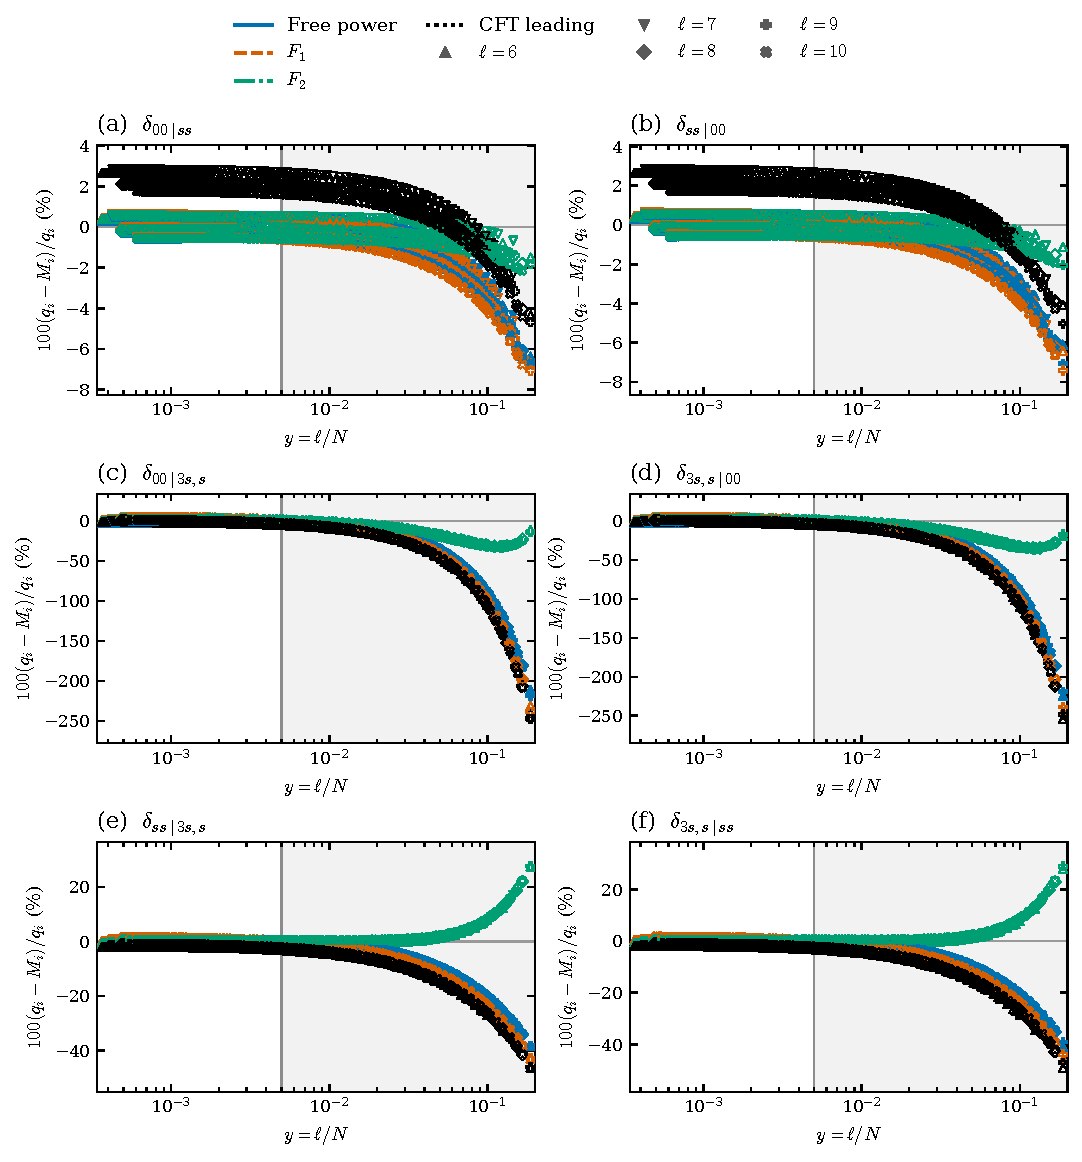
\includegraphics[width=.88\linewidth]{../figs/boson_large_residual.pdf}
\caption{The ordinate is $100(q_i-M_i)/q_i$ percent, with $q_i=D^A_i$ for a small interval and $q_i=\delta_i$ for a large interval; the horizontal zero line aids comparison. All four models have residual markers, colored as their curves. The residual ordinate is linear; the fraction axis is logarithmic. Compact-boson mixtures at $p=1/2$, $\ell=6,7,8,9,10$, and the chain-size set in Eq.~\eqref{eq:extended-grid}, with $32\leq N\leq16384$. There are 625 displayed geometries per direction at $y\leq0.2$, of which 317 satisfy $y\leq0.005$ and enter every fit. Marker shape identifies $\ell$; the vertical boundary and gray shading mark the fitting cutoff and excluded data. The boson uses $s=1/\sqrt2$, $q=2$, charge codes $(0,0),(1,1),(3,1)$, $z_j=e^{2\pi i j/N}$, $w_1=0$, and $W=10^8$; moment algebra uses 100 digits through $N=256$ and 120 digits at the added sizes. Natural logarithms apply. Added sizes use the direct entropy remainder in Sec.~\ref{sec:stable-entropy}, with support cutoff $10^{-15}$. Blue solid is the free-power fit (two fitted parameters), orange dashed is $F_1$ (one), green dash--dot is $F_2$ (two), and black dotted is the analytical CFT leading term (zero). Powers and amplitudes use Eqs.~\eqref{eq:fit} and \eqref{eq:complement-fit}; all coefficients include powers of $\pi$. Fits minimize unweighted squared residuals in $\delta$. These curves use \texttt{scaling\_fit\_summary.csv}. The identical fits in Tables~\ref{tab:boson-large-parameters} and \ref{tab:boson-large-metrics} also have per-pair full-range and fitting-window views in Sec.~\ref{sec:pair-large_boson}.}
\label{fig:boson-complement-residuals}
\end{figure}

